\chapter{Overview}

\section{The pre-2013 story}
\textit{The following is a concise summary of exploration between 1974 and 2012.All intervening expeditions and findings are described in greater detail in The Hollow Mountain volumes I and II}

\subsection{1974-1994 --- The early days} The JSPDT members initiated exploration around \passage{Migovec} in 1974, with the logging of 17 caves entrances (\passage{M1} through to \passage{M17}). There were two notable findings: \passage{M2} - pushed from 1974 to 1978 - and \passage{M16} -pushed from 1982 and 1985, which at -350m and -547m were the then deepest caves of Yugoslavia, and contained a huge underground cavern named \passage{Galaktika}. After 1985, the JSPDT focused their man power on exploring the \passage{Mala Boca} resurgence. \passage{Migovec} was left virtually untouched for another decade. 


	\begin{marginfigure}
    \vspace{-250pt}
	\checkoddpage \ifoddpage \forcerectofloat \else \forceversofloat \fi
	\centering
	\frame{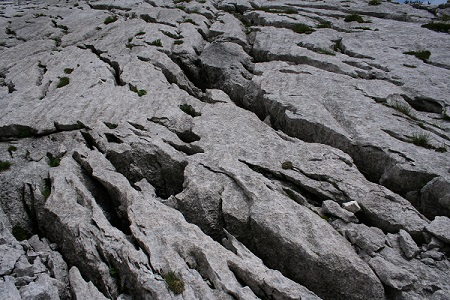
\includegraphics[width=\linewidth]{images/overview/jana_limestone.jpg}} 
  	\caption{A limestone pavement is where the story begins for the water, not so for cavers who prefer larger entrances to a cave system --- Jana \v{C}arga}
	\end{marginfigure}

\subsection{1994-2000 --- ICCC arrives in Slovenia} The first ICCC expedition to \passage{Migovec} took place in 1994; notable discoveries included \passage{M18} (cave of the \passage{Torn T-Shirt}), then 78m deep. The return visit in 1995 saw significant horizontal development (\passage{NCB passage}) and the set-up of a shallow underground camp (\passage{Club Mig}). This paved the way for several breakthroughs the following year and connection of \passage{M2}, \passage{M18} and \passage{M16}. 

\passage{Sistem Migovec} was born...

The following years saw a consistent probing of half a dozen different shaft series accessed by one single trunk route. Of these, only one (\passage{XXX}-\passage{Sajeta}) accessed deeper levels. Underground camping at \passage[camp]{Hotel Tolminka}.

\subsection{2000-2006 --- A new deep cave} In the year 2000 \passage{Vrtnarija} or \passage{Gardeners' World} entrance, which had been found several years earlier was dug out to reach a tight squeeze overlooking a loose pitch. Over the following days, pitch after pitch the cave continued gradually getting larger until \passage{Pico} pitch was discovered. This 10m diameter shaft plunged right into the heart of the mountain and carried both a strong draught and an anomalous amount of water. 

Below \passage{Pico}, the 2000 and 2001 expeditions explored a clean-washed and well-watered shaft series spanning -200 to -500m, past some smaller pitches to reach \passage{Zimmer} (P50). At the bottom a horizontal passage beckoned: \passage{The Gallery of Anglo-Slovene Friendship}. Some 400m of easy passage, following the chilling draught then led to a black void, the tantalising limit of exploration for 2001.
    
We set up an underground camp camp in \passage{Friendship Gallery} in 2003 and set out to descend the new pitch \passage{Big Rock Candy Mountain}, and the passages below. Over the next two years, the abandoned, sandy fossil passages at depths between -700m and -800m led north into hitherto completely blank mountain, ending at a terminal looking sump, underneath \passage{Tolminski Kuk}.

During the 2004 derig --- a process where the ropes of the entrance series were brought up the pitches, and metalwork taken out the cave --- Tetley spotted a window off the side of \passage{Pico}, bolted a route and swung into what appeared to be an excellent new, shallow lead. The 2005 expedition focussed on this branch. Awkward pitches and tight passages were the bread and butter of \passage{Captain Kangaroo} explorers and was left as a major lead after an aborted camping trip toward the end of the expedition.

	\begin{marginfigure}
    \vspace{-250pt}
	\checkoddpage \ifoddpage \forcerectofloat \else \forceversofloat \fi
	\centering
	\frame{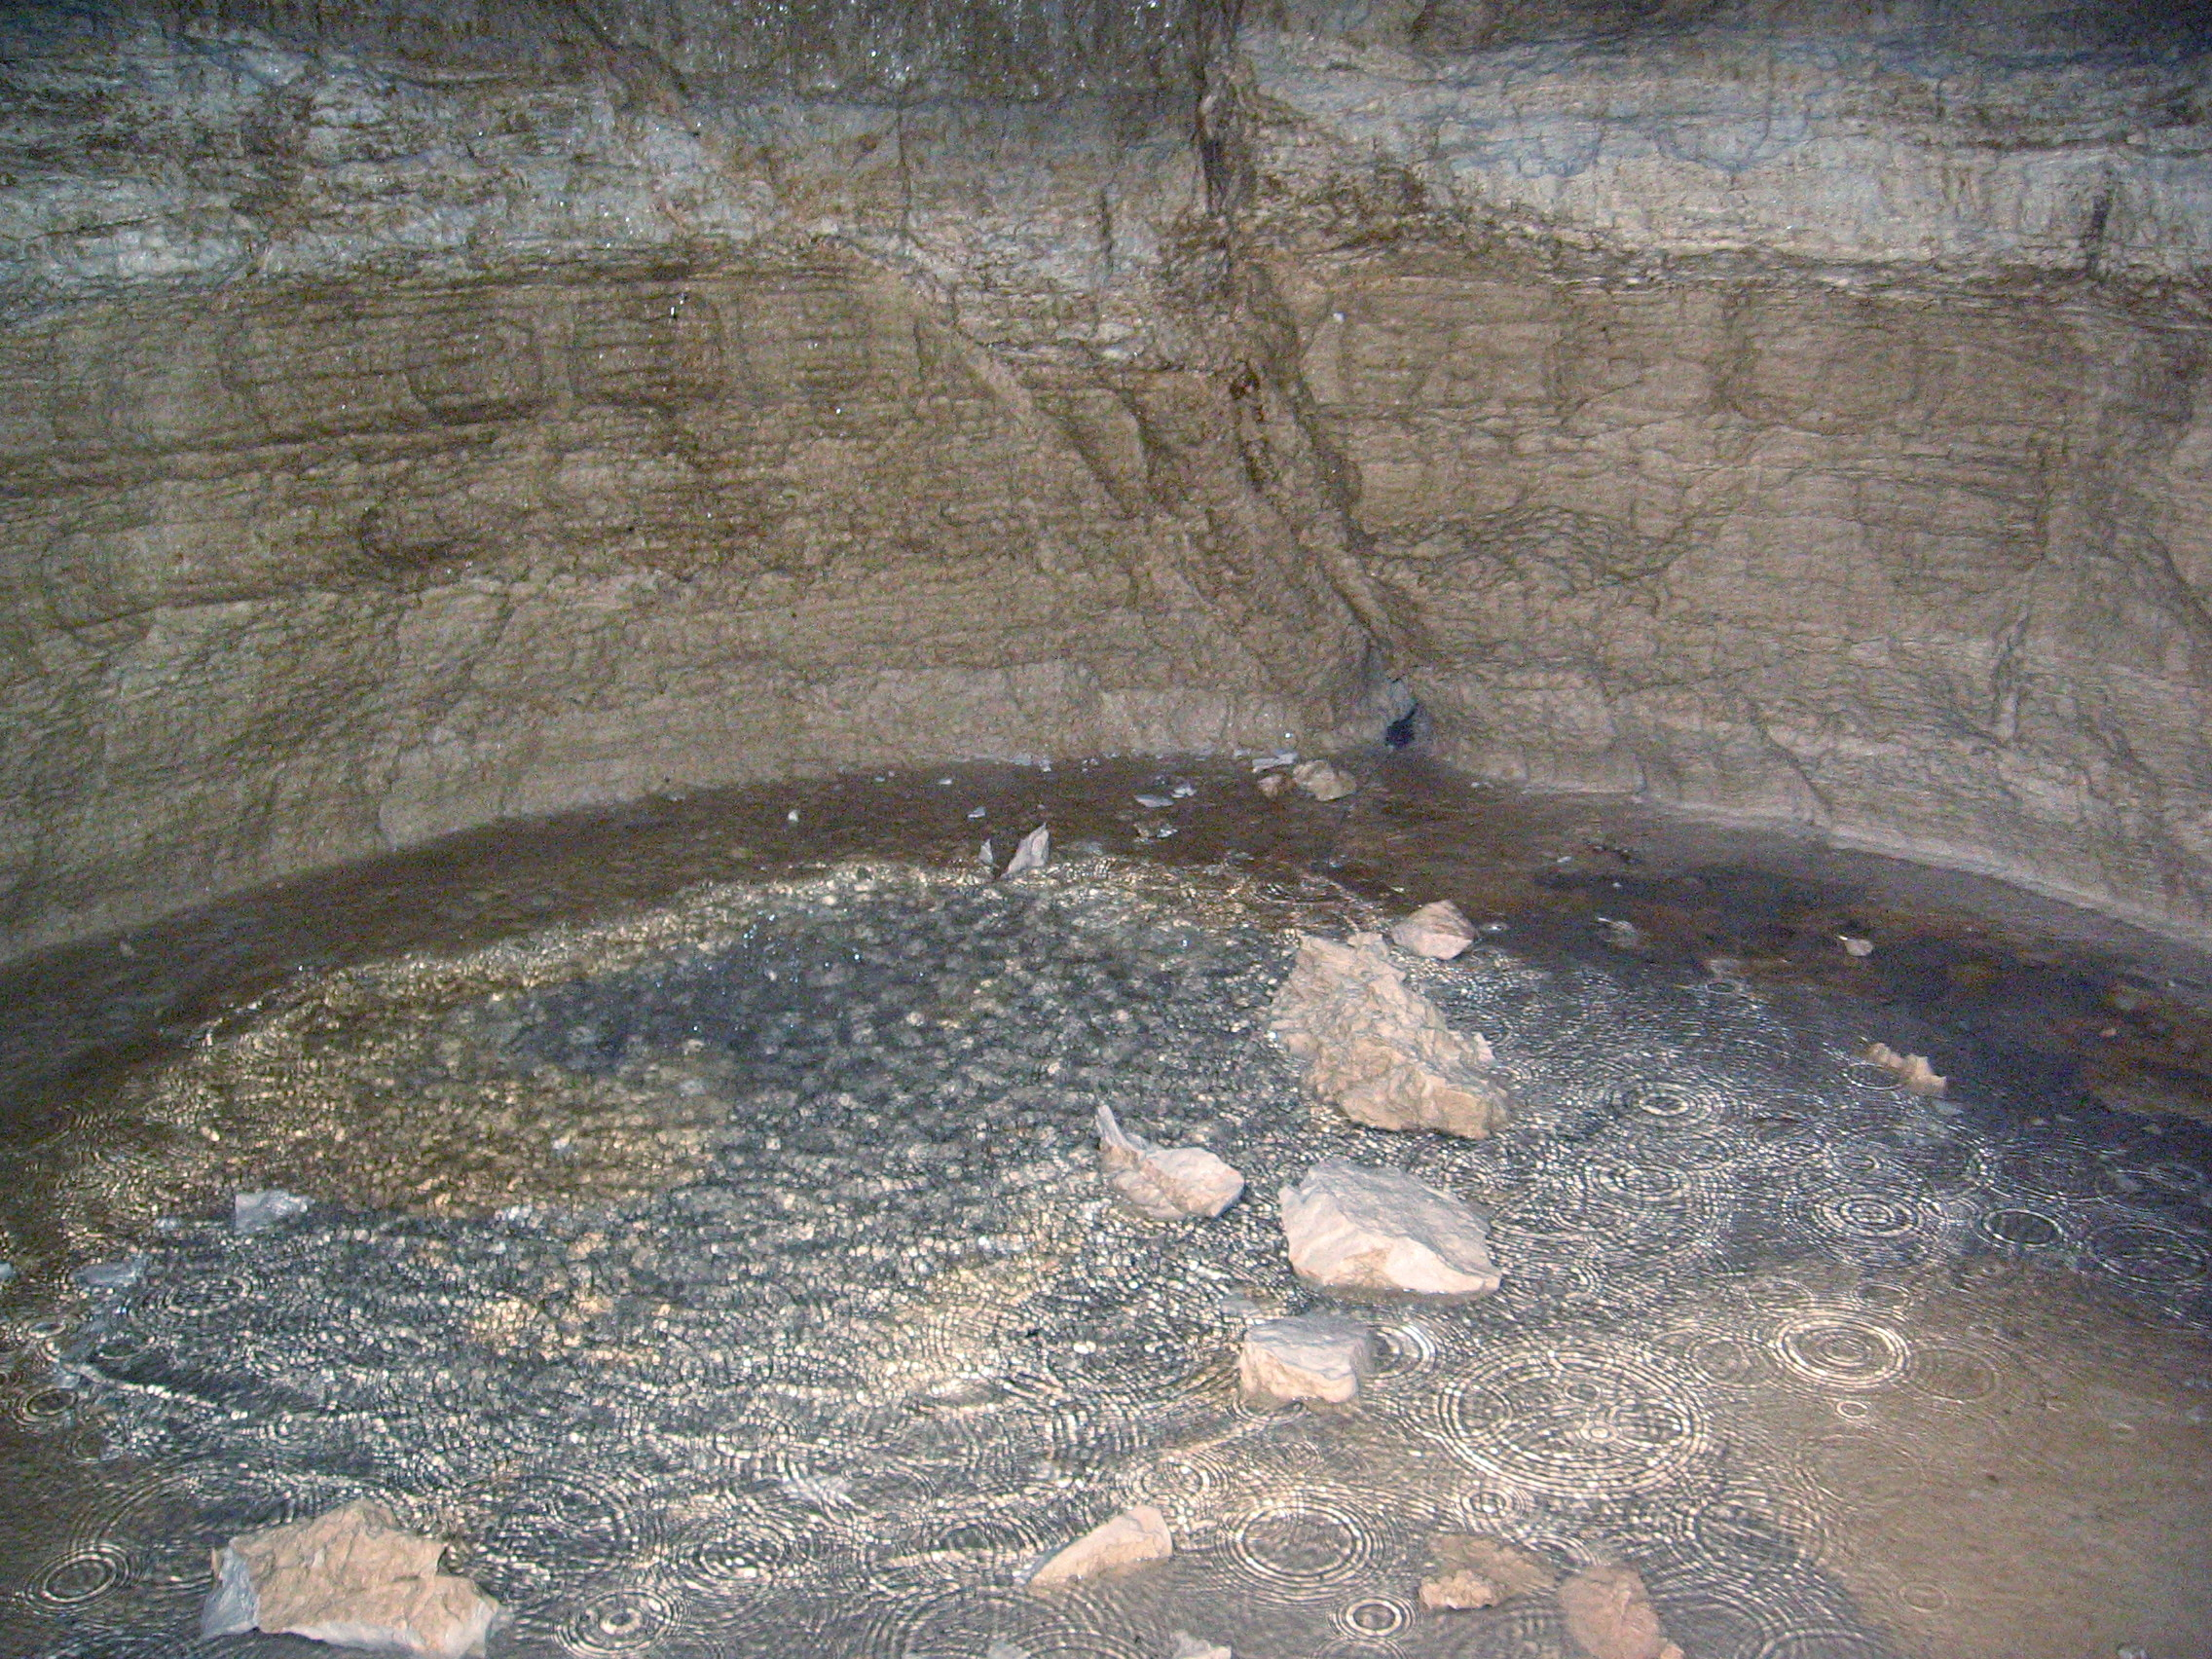
\includegraphics[width=\linewidth]{images/maps-of-mig/alchemy_drips_jana.jpg}} 
  	\caption{The bottom of \protect\passage{Alchemy} in \protect\passage{Vrtnarija} with is conspicuous flat floor and significant amount of water --- Jana \v{C}arga}
	\end{marginfigure}
    
    
\begin{marginfigure}
	\checkoddpage \ifoddpage \forcerectofloat \else \forceversofloat \fi
	\centering	\frame{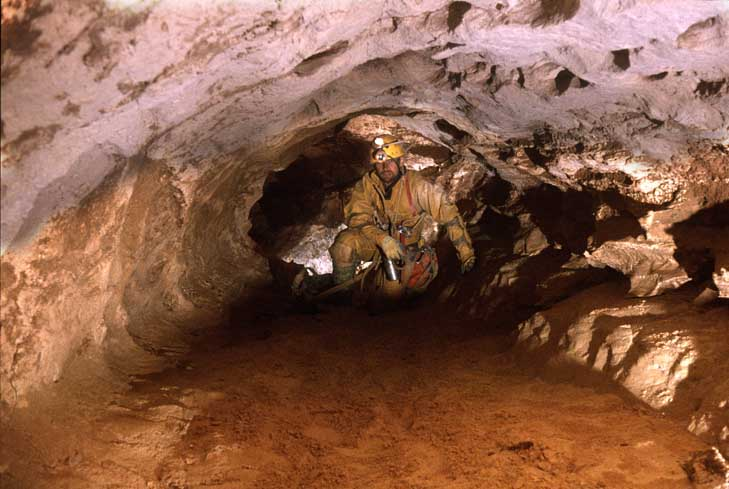
\includegraphics[width=\linewidth]{images/maps-of-mig/dw_highway32_oxbow.jpg}} 
  	\caption{The 2003-04 expedition findings included a plethora of interconnected passages below \protect\passage{Big Rock Candy Mountain} such as the sandy oxbow overlooking \protect\passage{Highway 32} streamway --- David Wilson}
	\end{marginfigure}

2006 was a year without ICCC summer expeditions, but Jarvist Frost and Jana \v{C}arga conducted an Autumn recce on the plateau, investigating the valleys to the west of the \passage{Plateau} as well as \passage{Area N}, a wilder plateau on the north side of \passage{Tolminksi Kuk}.

\subsection{2007-2009 --- Hard toil in Captain K branch} With plenty of new surface leads to push, the years 2007-2008 saw a concerted effort to find the next 'big cave' under the mountain. In parallel, the \passage{Captain Kangaroo} branch was extended further and found to head towards the bottom of \passage{M2} cave raising hopes for a connection between \passage{Vrtnarija}and \passage{Sysmig}, bringing the combined cave to just over 20km, thereby forging the second longest system in Slovenia as a reward for 15 years of nearly continuous exploration.

In 2009, \passage{Metal Camp} was set up in the newly found passages of \passage{Kill'em all}. Whilst no connection to M2 was made, the pitches increased in size again (\passage{Wet Hammer}, \passage{Mirage Canyon}, \passage{Happy Monday}), and dropped back to -550m, where a connection with \passage{Friendship Gallery} was forged. 

\subsection{2010-2012 --- A return to the deep Vrtnarija} 
\passage{M2} was revisited, its closest approach to Vrtnarija artificially enlarged over the course of several years. The two caves were well within survey error but no way through was found. 

Meanwhile, \passage{Friendship Gallery} was again used as a camp site location. On the back of the new improvements brought along with Metal Camp and with a 4 person hot-bedding system in place \passage{Camp X-Ray} became a palatial location: this played no small part in supporting true, deep alpine exploration.

From \passage{X-Ray} the cave was extended in three directions:
\begin{citemize}
\item Below \passage{Zimmer}, the \passage{Tolminka Korita}.
\item Below \passage{Cheetah}.
\item Towards the \passage{Royal Albert Hall}
\end{citemize}\passage{Palace of King Minos} branch 
    
\begin{marginfigure}
	\checkoddpage \ifoddpage \forcerectofloat \else \forceversofloat \fi
	\centering	\frame{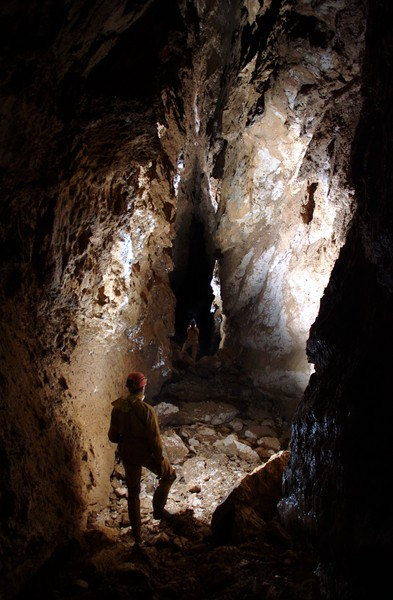
\includegraphics[width=\linewidth]{images/maps-of-mig/minotaur_rift_jarvist.jpg}} 
  	\caption{The \protect\passage{Minotaur Rift} was one of the findings of 2010, and one key element of the fossil passage series that ended connecting \protect\passage{Vrtnarija} and \protect\passage{Sysmig}--- Jarvist Frost}
	\end{marginfigure}

%\lettrine{S}{istem} Migovec, tucked away at the western edge of the Trigavski Narodni Park is the longest cave system in Slovenia. It has been since 2012, when, defying the expectations after a half a decade of effort, the connection between the ‘Old System’ (M2-M16-M18) and the newer Vrtnarija (Gardener’s World) and Vilinska Jama cave was forged after a routine pushing trip at -600m. This - 38 years since the beginnings of exploration underneath Tolminski Migovec, ‘Mig’ as it is affectionately named - made the national news. 

%Since then, and rather more discreetly,  Imperial College cavers (ICCC) have repeatedly spent their summers discovering more voids under the hollow mountain, in tandem with the Jamarska Sekcija Planinskega Drustva Tolmin (JSPDT). Bit by bit, the other pieces of the puzzle were extended and connected to the main system. In October 2015, three Slovene cavers found a way between the last big independent cave system, Primadona-Monatip-Uben571 and one of the earliest high level passages of Sistem Migovec, bringing the total to 35.6km of connected passage. Since October 2017, it stands at 39.2km.

\section{2013 --- We’re not alone}

When the reports of a live creature sighting came back to the surface, they were first met with disbelief. Tetley, one of the long standing members of the expedition and Sam Page, a then second year student had spent several days underground, poking at the previous year’s ‘connection’ passages, hoping that in the rush for the finish line, side passages may have been missed. Since 2010, the expedition relied on camping in the \passage{Gallery of Anglo-Slovene Friendship}, a horizontal, abandoned phreatic 550m below the surface, a gallery from which it was possible to access the rapidly expanding pushing fronts under 3 hours. The entrance series to the cave was relatively hassle-free and direct, barring the ultimate pitch, whose spectacular free-hanging descent was ever so slightly wet, but this had its own advantages: it provided a ready source of water and untapped washing power; indeed any cutlery and cooking pots left for a couple of hours would inevitably come out spotless.

\begin{marginfigure}
	\checkoddpage \ifoddpage \forcerectofloat \else \forceversofloat \fi
	\centering	\frame{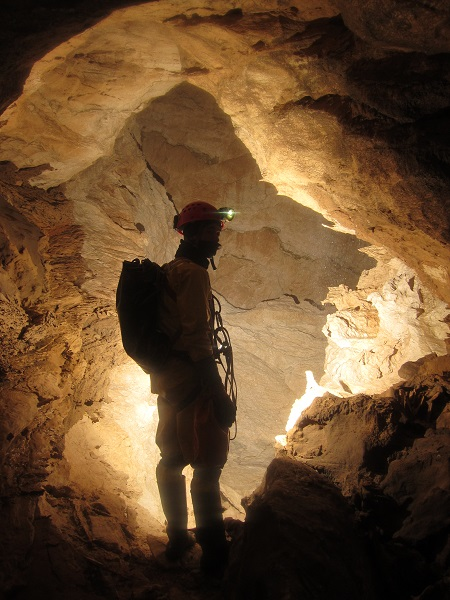
\includegraphics[width=\linewidth]{images/overview/rhys_red_cow.jpg}} 
  	\caption{A lot of the 2013-2015 exploration took place in the deep \protect\passage{Vrtnarija} levels --- Jarvist Frost}
	\end{marginfigure}

It was from this palatial camp that the exploratory duo went for a visit to the southern branch of the system, a series of muddy, but essential bone dry, strongly draughting and horizontal galleries. Recent extensions were headed due south, along an old phreatic tunnel, modified by breakdown in places, and, extraordinarily for this particular alpine system, decorated with stalactites. The encounter happened at one of the rare spots where water trickles in from the roof, right at the foot of an extremely muddy pitch. They caught a glimpse of a live dormouse, furry tail and all, right at the heart of the mountain and lived to tell the tale. Where had it come from? 

While this question did not fuel a mad break for the surface, steady exploration of the southern branches by Rhys Tyers, Dave Kirkpatrick, Clare Tan and myself over the following years yielded more and more evidence that these mammals do occasionally wander into and litter our cave system.

\section{2014-2015 --- The cave goes South}

In 2014, we went further into the \passage{Atlantis} branch, finding a sizeable stream at the far end of the large, sediment filled \passage{Helm’s Deep} chamber. The interest went soon over to a north-south oriented rift, draughting very strongly outwards and heading towards the southern face of \passage{Tolminski Migovec}. This puzzled us for a while: a vertical maze of climbs and drops where metres of passage were hard won. There, we first found the mouldy remains of dormouse at the foot of a small climb. For want of rope and time, we left this for the next expedition to resolve.



2015 saw us eager to find a way out of the cave: the first trip had found more rift, bringing the surface to fewer than 500m horizontally. On the surface, Jack Hare plotted the known end of the cave against the topographical map, and with rough coordinates in the GPS set out to discover the lower entrance. This was successful: by climbing up a N-S oriented canyon, he and Rhys stumbled upon a possible opening which had a good draught, whistling through a mud and boulder blockage. 

\begin{marginfigure}
	\checkoddpage \ifoddpage \forcerectofloat \else \forceversofloat \fi
	\centering	\frame{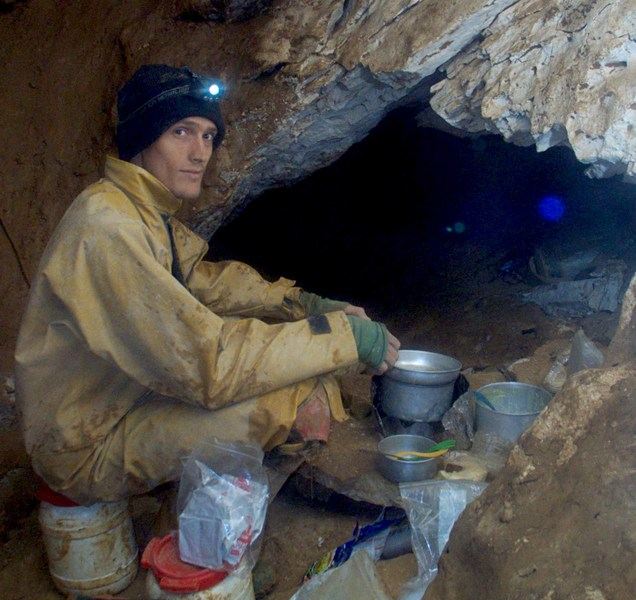
\includegraphics[width=\linewidth]{images/maps-of-mig/jarv_at_camp_mugshot.jpg}} 
  	\caption{2014-15 saw more action from camp \protect\passage{X-Ray}--- Jarvist Frost}
	\end{marginfigure}

I arrived late on the expedition, but soon got underground with Rhys, motivated to push the southern end as well. We quickly broke through a choke, descended a 25m pitch where I pointed out the exposed fault planes which had obviously guided its current morphology, and at the bottom rejoined the main, abandoned phreatic level, stretching all the way to \passage{Atlantis} for more than a kilometre. This led us south, and excited as we were to be treading the easy walking passage of the \passage{Meridian Way}, we couldn’t help but notice scratch marks, hair, bones and excrement littering the gallery floor. The next team pushed this even further, getting to within 250m from the surface. Next up was a constriction that would need time and effort to pass.

But this was it for the lower entrance story: turning back from that part of the cave, we had 4-5hrs caving to reach the camp, and that again to get back out on the surface. At the end of the summer 2015, we collectively decided to shift our objectives and luckily, a completely new training ground had opened up to us.

\section{2000-2015 --- The twelve battles of Monatip}
Back in the early 2000’s, while ICCC were busy pushing \passage{Vrtnarija}, entering the mountain from the eastern side, cavers from the JSPDT investigated a large entrance situated half-way down the western cliff, named \passage{Primadona}. Early day trip explorations extended the cave to over 600m in depth, and it wasn’t until 2007 that another entrance  on the cliffside, roughly 100m north was spotted: this became \passage{Monatip} cave. The system proved a training ground for the younger members of the JSPDT from 2008 onwards, after these two western caves were connected. Exploration picked up in earnest after the well publicised 2012 connection as the added 5km of \passage{Primadona}-\passage{Monatip}-\passage{Ubend571} would put \passage{Sistem Migovec} out of reach of its more famous contender, \passage{Postojnska Jama}, but many cavers doubted there could be a connection, due to a large surface fault, coinciding with hitherto unexplored, blank mountain. The way did exist however.

One of the key members of the later exploration of \passage{Monatip} was Dejan Ristic, who, over the course of twelve assaults, therefore mirroring the more sinister WWI Soča battles, forged the connection between \passage{Monatip}, and \passage{Sistem Migovec}. Together with Andrej Fratnik, long-standing \passage{Migovec} explorer and Iztok Mozir, they traversed, and squeezed and dug, and eventually emerged in \passage{NCB} passage. This ground, first tread in 1995 by ICCC cavers had proved time and again critical in the connection stories of the \passage{Migovec} caves, its discovery playing no small part in the early survival of the IC expeditions. The successful trio fittingly exited via \passage{M2}, the oldest explored entrance which is kept permanently rigged.

	\begin{marginfigure}
	\checkoddpage \ifoddpage \forcerectofloat \else \forceversofloat \fi
	\centering
	\frame{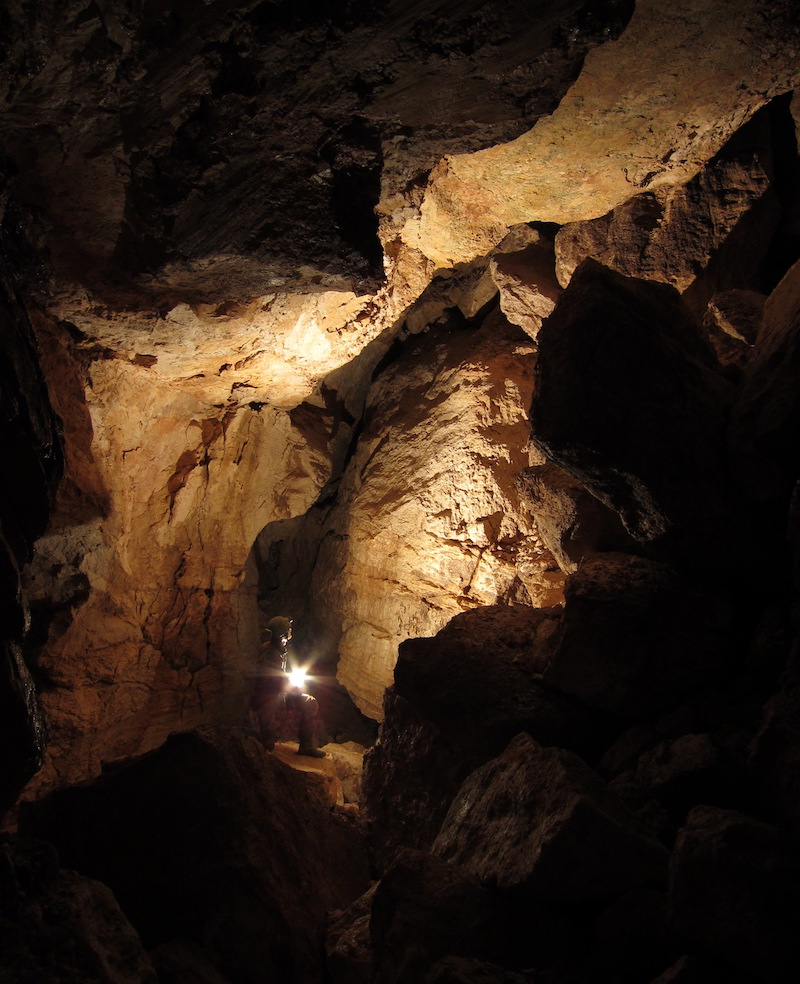
\includegraphics[width=\linewidth]{images/2017/tanguy-hammerhead-2017/hammerhead-chamber.jpg}} 
  	\caption{Discovery of \protect\passage{Hammerhead} chamber one of the later findings of 2017 --- Jarvist Frost}
	\end{marginfigure}

\section{2016 --- The road less traveled}
This is how things stood in the closing months of 2015. Plans to move to the deeper, and possibly still fertile ground of \passage{Primadona} were formed. Some of the newer expedition members, myself included wanted to start bolting deeper pitches, and the rerigging project we formulated provided just that. We would be able to take novices on easier bounce trip, allured by the promise of shallow leads left unpushed in a bid for greater depth.

The cave, while far from perfect provided many surprises. For almost all of the IC cavers, this was \textsl{terra incognita}  from the onset. Why, it took us four days, and an aborted attempt down the wrong valley to locate and reach the entrance. By that time, I’d put in more bolts with a drill than for two previous expeditions, but then, we got some help from the JSPDT. Zdenko, aside from bringing the appreciated \v{Z}ganje and local deer sausage, showed us the way on, giving names to places, which we shamefully Anglicised. \passage{Sejna Soba}, the meeting room, became ‘\passage{Sane and Sober}’ something Migovec cavers as a whole cannot be accused of being. He showed and pointed at openings ‘I’ve never been, we think it goes towards X… always go left you will find blank mountain...’ Clearly, there was potential.


\begin{marginfigure}

	\checkoddpage \ifoddpage \forcerectofloat \else \forceversofloat \fi
	\centering
	\frame{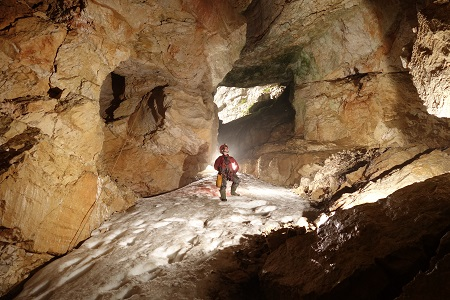
\includegraphics[width=\linewidth]{images/overview/rhys_diss_prima.jpg}} 
  	\caption{The relatively large entrance chamber of \protect\passage{Primadona} collects winter snow --- Rhys Tyers}
	\end{marginfigure}

We pooled our newly gained knowledge of the cave and to our surprise we started treading new ground: pitches which had been rigged but not descended, obscure climbs which led to vast caverns, a parallel shaft series which we connected back to the old way down deep. And somehow, the old objective of going down deep was forgotten: we were side tracked at every level by a complex series of connected, horizontal passages. Yet, the almost mythical left turn into blank mountain eluded us.

\section{2017 --- Divine intervention}
The 2017 team approached the cave differently. For the returning cavers, the novelty had worn off, we’d mulled over our best leads during eleven months, and we were keen to make our knowledge count. So we almost tacitly concentrated our efforts to three areas of \passage{Primadona}: the \passage{Galerija}, \passage{TTT} and \passage{Fenestrator} branches.

The \passage{TTT} branch, which I’d become familiar with in 2016 was the original way to the deepest point of \passage{Primadona}. A side passage which I’d spotted led to a series of chambers and pitches, ending in a draughting, high aven where the boulder collapse was pervasive. We ran out of steam there: the trips were long and strenuous, the cave never particularly friendly.

Over to the west, Jack Hare bolted a metal-rich traverse over a 40m drop to gain the continuing horizontal passage at the far end of \passage{Galerija}. This was very successful and promising: a memorable push led to increasingly large pitches (P5, P10, P22), ending at yet another drop. Eventually, this provided a stunning abseil through the roof of the \passage{Hall of the Mountain King} (P42), a cavern found the previous year: the exploration met a satisfying end.

It was further up the cave, very close to a small rest-stop we’d set up - and nicknamed \passage{Mary’s Caf\'{e}}- that the most significant discoveries of the year took place. Little by little, an obscure SE trending rift led away from the main tangle of passages. Ever changing in nature, now a muddy phreatic (\passage{Plumbers' Paradise}), now a vadose stream (\passage{Hallelujah}), now a clean-washed pitch series (\passage{Sweet Baby Jesus}), this branch extended far into the blank mountain we’d been advised to explore.  

\begin{marginfigure}
\vspace{-200pt}
	\checkoddpage \ifoddpage \forcerectofloat \else \forceversofloat \fi
	\centering
	\frame{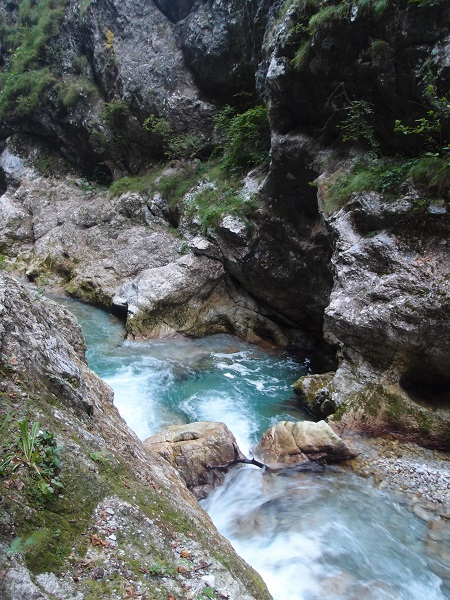
\includegraphics[width=\linewidth]{images/overview/tolminka_cecilia.jpg}} 
  	\caption{Precipitation in the high limestone ranges finds its way underground and resurges as two stunningly blue streams: the \protect\passage[river]{Tolminka} and \protect\passage[river]{Zadla\v{z}cica} rivers, photographed near their confluence --- Cecilia Kan}
	\end{marginfigure}

\section{The outlook}
So what next? There's plenty of interest for the upcoming the 2018 expedition, where we hope to be camping in \passage{Primadona} and finally push the deeper levels. One thing is for certain, the successful annual expeditions have helped cement a true club spirit and prepare the newer cavers for the leadership roles they naturally assumed coming back to the UK. 

\name{Tanguy Racine}
